\chapter{Related Work}
\label{chap3}



A parallel study was conducted by Qamar et al. \cite{atmospheric-correction-refl}. The objective of this work was to recover true vegetation reflectance, with the primary inputs being the spectral radiance captured by a ground-based remote sensing system and the time and date when the data were collected, without knowing the exact atmospheric conditions present during data collection. Previously implemented algorithmic methods tend to either be highly computationally inefficient, in the case of radiative transfer approaches, or to introduce large uncertainties, depending on the amount of context they are provided with. ML methods, as shown in the work, tend to be relatively computationally efficient while also maintaining a degree of accuracy, even when information such as atmospheric parameters, which in other cases would be necessary, is absent.

To meet the data requirements, the researchers relied heavily on synthetic data. Specifically, they combined simulated vegetation reflectance with simulated atmospheric and solar effects, acquiring the associated at-sensor radiance in the process.  Subsequently, they introduced artificial noise to represent sensor artifacts.

The produced data were used for training a series of Convolutional Neural Networks. The models, given the distorted radiance, output $\Delta reflectance$, the ratio of vegetation reflectance to the median simulated spectrum, which is then used to reconstruct the final reflectance curve. The overall process of data synthesis, model training, and reflectance reconstruction is illustrated in Figure~\ref{rwRef}.

Eventually, the models achieved an $R^2$ of $0.981 \pm 0.004$ when predicting simulated reflectance values. For real-world measurements, the researchers compared the relative reflectance changes predicted by ten independently trained models, expressing a range of uncertainty, with those obtained using the Compound Ratio method. The results showed similar trends in the relative reflectance changes obtained by the two methods.

\begin{figure} [htb]
    \centering
    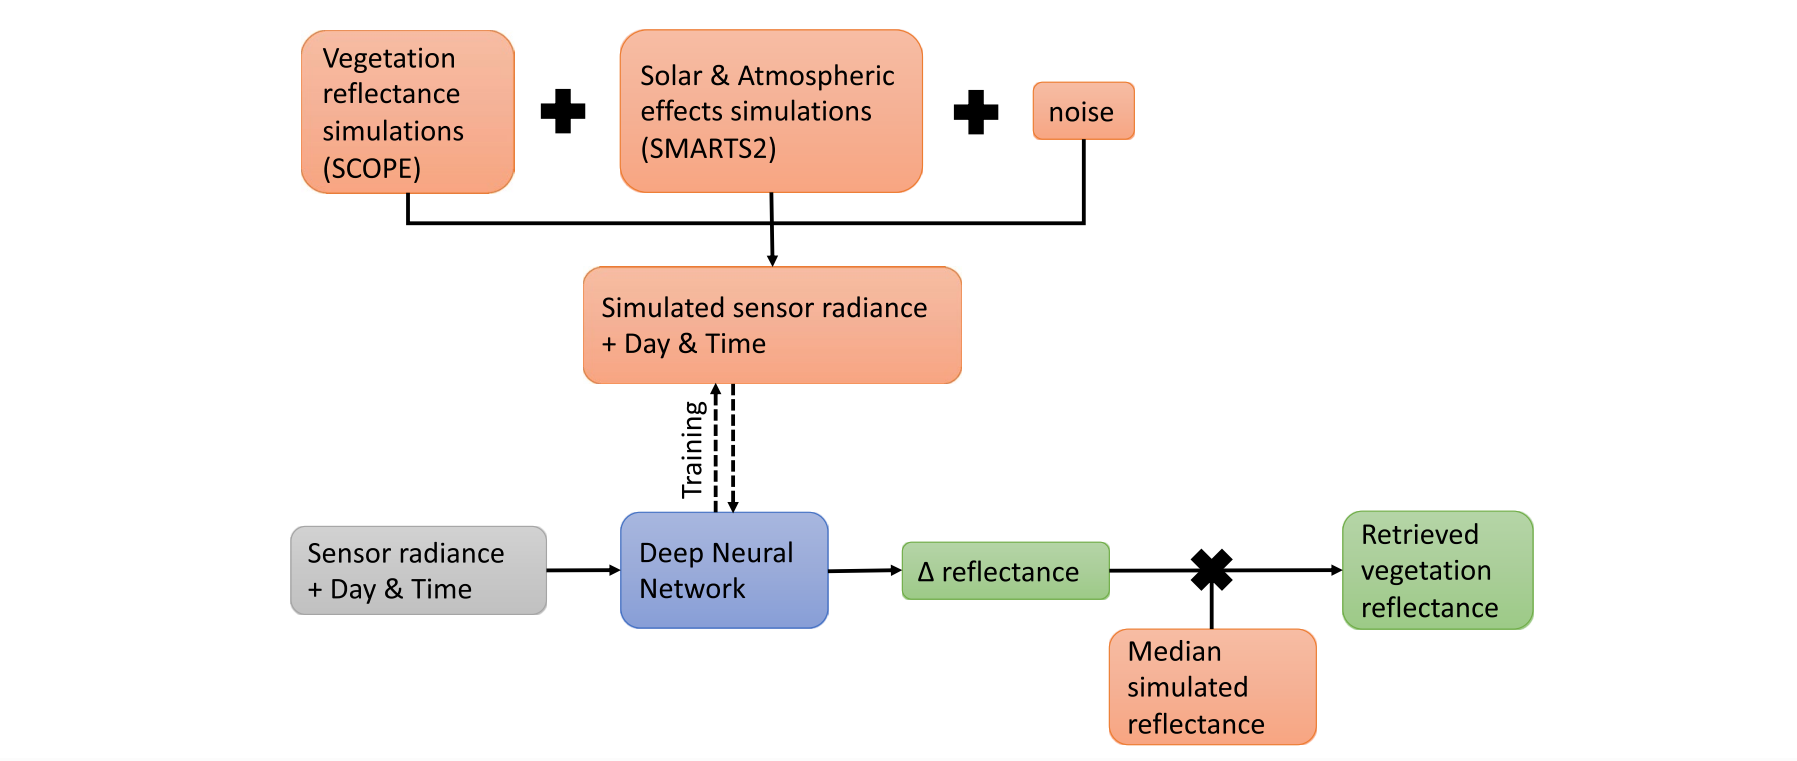
\includegraphics[width=1\linewidth]{images/related-work-1.png}
    \caption{Figure included in \cite{atmospheric-correction-refl}. Depicts an overview of the deep learning framework for retrieving vegetation spectral reflectance from hyperspectral measurements.}
    \label{rwRef}
\end{figure}

Another closely related work was performed by Jasso-Garduño et al. \cite{dl-based-emul}. Within this study, several Deep Neural Network architectures were developed that, given information about the sun-sensor geometry, apparent radiance and Aerosol Optical Depth, were trained to approximate the Earth's surface reflectance. The main motive is to provide an alternative to the computationally expensive radiative transfer methods. The data used for the training of the models were generated using 6S, a radiative transfer model designed to simulate how sunlight interacts with the atmosphere. The best performing model achieved an $R^2$ of $0.995$ when approximating the simulated values. It is important to mention that this this performance was achieved within a specific range of input values, and might need retraining to retain this performance across other scenarios. 


Other related works include those of Siddiqua et al. \cite{macgan} and Joiner et al. \cite{noise-reduct-solar-ind}. In the first one, a Generative Adversarial Network was trained using synthetic data to remove distortion introduced to images by weather phenomena and underwater conditions. In the latter,  ML is used to reduce noise from satellite measurements of terrestrial chlorophyll solar-induced fluorescence. Both simulated and non-simulated data were used for training.

The common source of error across all the aforementioned studies is the influence of uncontrollable parameters when capturing data in outdoor environments, primarily related to atmospheric phenomena and variations in sun-sensor geometry. As in the present study, the proposed solutions for approximating metrics under the desired conditions involve the use of ML models. Given the large amount of data required to train and evaluate such algorithms, the satisfactory performance of models trained on synthetic data and their transferability to real-world data inspired the use of simulations as a data source in the present study.